\section{Introduction}
A major challenge in reinforcement learning is to design agents that are able to learn efficiently and to adapt their existing knowledge to solve new tasks. As it has been discussed, one way to reduce the complexity of learning is hierarchical reinforcement learning~\citep{Sutton1999, Dietterich2000, Barto2003}. Here a novel approach to hierarchical reinforcement learning in LMDPs that takes advantage of the compositionality of LMDPs is proposed. This approach assumes that the state space is partitioned into subsets, and the subtasks consist in moving between these partitions. The subtasks are parameterized on the current value estimates of boundary states. 
In section~\ref{section:compositionality}, compostionality was shown to be one of the computational advantages of LMDPs, which allows for zero-shot learning of new skills by linearly combining previously learned base skills which only differ in their cost or reward at boundary states~\citep{Todorov2009,Silva2009}. 

In this work, instead of solving the subtasks each time the value estimates change, the compositionality property of LMDPs is exploited to express the solution to an arbitrary subtask as a linear combination of a set of base LMDPs. The result is a form of value function decomposition which allows expressing an estimate of the optimal value of an arbitrary state as a combination of multiple value functions with smaller domains.

In this chapter, two algorithms are proposed, the first is a two-step eigenvector when both the passive dynamics and the reward functions are known. When these are unknown to the learning agent, an online algorithm can be used to simultaneously learn the value function of the subtasks and the value for the boundary states. Emprical results accompany these theoretical formulations.
\section{Contributions}
\begin{itemize}
%\item We define a novel scheme based on compositionality for solving subtasks, defining local reward functions that constitute a convenient basis for composite reward functions.
\item To define a novel scheme based on compositionality for solving subtasks, defining local rewards that constitute a convenient basis for composite rewards.
\item The subtask decomposition is at the level of the value function, not of the actual policy. Hence the proposed approach does not suffer from non-stationarity in the online setting, unlike approaches that select among subtasks whose associated policies are being learned.
\item Even though the subtasks have local reward functions, under mild assumptions the proposed approach converges to the globally optimal value function.
\item The proposed learning algorithm is analyzed empirically and it shows in two classical domains 
that it is more sample efficient compared to a flat learner and similar hierarchical approaches when the set of boundary states is smaller than the entire state space.
\end{itemize}


\section{Related Work}
Several authors have recently exploited concurrent compositionality of tasks in the context of transfer learning.~\citet{Niekerk2019} use the linear compositionality of LMDPs to solve new tasks that can be expressed as combinations of a series of existing base tasks. They show that, while disjunctions of base tasks (OR-compositionality) can be performed exactly, the AND composition (when the goals of base tasks partially overlap) can only be performed approximately.

\citep{Haarnoja2018a} exploit a similar idea to transfer knowledge from existing tasks to new tasks by averaging their reward functions.~\citep{Hunt2019} further extended this by introducing the so-called compositional optimism, and apply divergence correction in case compositionality does not transfer well.

More recently, \citep{NangueTasse2020} derive a formal characterization of union and intersection of tasks in terms of Boolean algebra. They show that learning (extended) value functions that account for all achievable goals, exact zero-shot transfer learning using both AND- and OR- compositionality is possible, achieving an exponential increase in skills compared to the previous works.

All the aforementioned results are derived for general MDPs with deterministic dynamics and, possibly, entropy regularization. This setting is no more general than the class of LMDPs.

%~\textit{van2019composing} use compositionality in systems with deterministic dynamics to solve new tasks that can be expressed as combinations of a series of existing tasks. The authors distinguish between AND-compositionality and OR-compositionality, depending on whether the features of a new task are present in all existing tasks or only some.
%and present a method that approximates AND-compositionality and 

%The above forms of compositionality do not guarantee that the resulting policy is optimal, unlike compositionality for LMDPs which is exact.
The aim of this work is to integrate both concurrent task composition, as done in the above approaches, together with hierarchical composition, where skills are chained in a temporal sequence, under the framework of LMDPs.

Several authors have proposed hierarchical versions of LMDPs.~\cite{Jonsson2016} extend MAXQ~\citep{Dietterich2000} to LMDPs by defining subtasks that represent high-level decisions. The top-level policy chooses multi-step transitions, which introduces non-stationarity in the high-level decision process if subtasks are learned concurrently, and also prevents global optimality. The authors discuss the idea of compositionality, but do not explore the concept further.
~\citet{Saxe2017} propose a hierarchical multi-task architecture that does exploit compositionality. Their multitask LMDP maintains a parallel distributed representation of tasks, reducing the complexity through stacking. However, the approach requires to augment the state space with many additional boundary (subtask) states. Further, the stacking introduces additional costs (cf. their Equation 10), and does not provide global optimality.

The options keyboard \citep{Barreto2019} combines a successor feature representation with generalized policy improvement to obtain subtask policies from a set of base subtasks without learning, similar to subtask compositionality used in the proposed method. However, unlike in this, their composition weights have to be set manually, and although the composed policy is guaranteed to be better than the individual base policies, it is not guaranteed to be optimal.

%\textit{multipl}

The proposed method is similar to that of \citet{Wen2020} since a hierarchical decomposition based on a partition of the state space is defined, and exploit the equivalence of subtasks to reduce the learning effort. Unlike previous work, however, the LMDP approach is not restricted to single initial states, does not suffer from non-stationarity in the online setting, proposes a more general definition of equivalence that captures more structure, and guarantees convergence to the optimal value function for stochastic dynamics.

The concept of equivalent subtasks is strongly related to factored (L)MDPs, which capture conditional independence among a set of state variables~\citep{Boutilier1995, Koller2000}. Equivalence arises whenever a subset of state variables are conditionally independent of another subset. Several authors have shown how to automatically discover the structure of factored MDPs from experience~\citep{Strehl2007,Kolobov2012}, which in turn could be used to define equivalence classes of subtasks.

%{\color{red} Mention here the other papers \textit{hunt2019composing}\textit{van2019composing},\textit{algebra}}

\section{Hierarchical LMDPs}

This section describes the novel approach to hierarchical LMDPs. First, there is a description of the particular form of hierarchical decomposition that is considered, and then the algorithms for solving a decomposed LMDP are introduced.

\subsection{Hierarchical Decomposition}

The hierarchical decomposition is similar to that of~\citep{Wen2020}. Formally, given an LMDP $\cL=\langle\cS,\cT,\kernel,\cR,\cJ\rangle$, the set of non-terminal states $\cS$ is partitioned into $L$ subsets $\{\cS_i\}_{i=1}^L$. For each such subset $\cS_i$, there exists an induced subtask $\linebreak {\cL_i=\langle\cS_i,\cT_i,\kernel_i,\cR_i,\cJ_i\rangle}$, i.e.~an LMDP whose components are defined as follows:
\begin{itemize}
\item The set of non-terminal states is $\cS_i$.
\item The set of terminal states $\cT_i=\{\tSi \in\cS^+\setminus\cS_i:\exists s\in \cS_i \; \text{s.t.} \; \tSi \in \cB(\kernel(\cdot|s))\}$ includes all states in $\cS^+\setminus\cS_i$ (terminal or non-terminal) that are reachable in one step from a state in $\cS_i$.
\item $\kernel_i:\cS_i\rightarrow\Delta(\cS_i^+)$ and $\cR_i:\cS_i\rightarrow\real$ are the restrictions of $\kernel$ and $\cR$ to $\cS_i$, where $\cS_i^+=\cS_i\cup\cT_i$ denotes the full set of subtask states.
%\item The reward of a terminal state $\tS\in\cT_i$ equals $\cJ_i(\tS)=\cJ(\tS)$ if $\tS\in\cT$, and $\cJ_i(\tS)=\widehat{v}(\tS)$ otherwise, where $\widehat{v}(\tS)$ is the estimated value in $\cL$ of the non-terminal state in  $\tS\in\cS \setminus \cS_i$.
\item The reward of a terminal state $\tSi \in\cT_i$ equals $\cJ_i(\tSi)=\cJ(\tSi)$ if $\tSi\in\cT$, and $\cJ_i(\tSi)=\widehat{v}(\tSi)$ otherwise, where $\widehat{v}(\tSi)$ is the estimated value in $\cL$ of the non-terminal state in  $\tSi\in\cS \setminus \cS_i$.
\end{itemize}

Intuitively, if the reward $\cJ_i(\tSi)$ of each terminal state $\tSi\in\cT_i$ equals its optimal value $v(\tSi)$ for the original LMDP~$\cL$, then solving the subtask $\cL_i$ yields the optimal values of the states in $\cS_i$.
In practice, however, an estimate $\widehat{v}(\tSi)$ of the optimal value is used.
% VG : what do you mean in practice: during learning? in the presence of function approximation?
In this case, the subtask $\cL_i$ is {\em parameterized} on the value estimate $\widehat{v}$ of terminal states in $\cT_i$, and each time the value estimate changes, $\cL_i$ can be solved to obtain a new value estimate
$\widehat{v}(s)$ for each state $s\in\cS_i$.



Let $\cE=\cup_{i=1}^L\cT_i$ be a set of {\em exit states}, i.e.~the union of the terminal states of each subtask in $\{\cL_1,\ldots,\cL_L\}$. For convenience, let $\cE_i=\cE\cap\cS_i$ denote the set of (non-terminal) exit states in the subtask $\cL_i$. Also, consider the notation $K=\max_{i=1}^L|\cS_i|$, $N=\max_{i=1}^L|\cT_i|$ and $E=|\cE|$.

The notion of subtasks is just like in~\citep{Wen2020}.
\begin{definition}
Two subtasks $\cL_i$ and $\cL_j$ are equivalent if there exists a bijection $f:\cS_i\rightarrow\cS_j$ such that the transition probabilities and rewards of non-terminal states are equivalent through $f$.
\end{definition}
Unlike \citep{Wen2020}, this definition does {\em not} require the sets of terminal states $\cT_i$ and $\cT_j$ to be equivalent. Instead, for each class of equivalent subtasks, the approach is to define a single subtask whose set of terminal states is the {\em union} of the sets of terminal states of subtasks in the class.

Formally, a set of equivalence classes $\cC=\{\cC_1,\ldots,\cC_C\}$ is defined, $C\leq L$, i.e.~a partition of the set of subtasks $\{\cL_1,\ldots,\cL_L\}$ such that all subtasks in a given partition are equivalent. Only a single subtask $\cL_j=\langle\cS_j,\cT_j,\kernel_j,\cR_j,\cJ_j\rangle$ needs to be represented per equivalence class $\cC_j\in\cC$. The components $\cS_j,\kernel_j,\cR_j$ are shared by all subtasks in the equivalence class, while the set of terminal states is $\cT_j=\bigcup_{\cL_i\in\cC_j} \cT_i$, where the union is taken w.r.t. the bijection $f$ relating all equivalent subtasks. As before, the reward $\cJ_j$ of terminal states is parameterized on a given value estimate $\widehat{v}$. It is assumed that each non-terminal state $s\in\cS$ can be easily mapped to its subtask $\cL_i$ and equivalence class $\cC_j$.


\begin{figure}[!t]
\begin{center}
        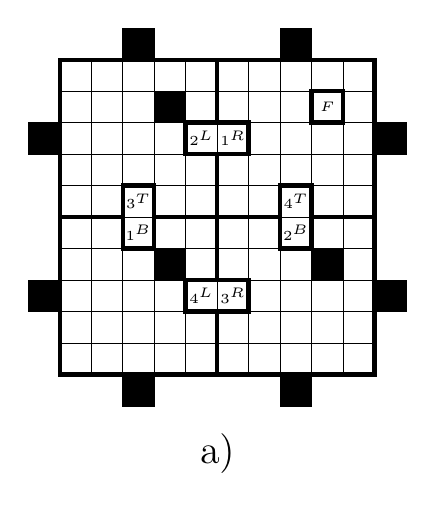
\begin{tikzpicture}
        \draw[step=0.4,thin,shift={(0.2,0.2)}] (0.8,0.8) grid (4.8,4.8);
        \draw[ultra thick] (1,1) rectangle (5,5);
        \draw[ultra thick] (3,1) -- (3,1.8);
        \draw[ultra thick] (3,2.2) -- (3,3.8);
        \draw[ultra thick] (3,4.2) -- (3,5);
        \draw[ultra thick] (1,3) -- (1.8,3);
        \draw[ultra thick] (2.2,3) -- (3.8,3);
        \draw[ultra thick] (4.2,3) -- (5,3);
        
        \draw[fill] (0.6,1.8) rectangle (1,2.2);
        \draw[fill] (0.6,3.8) rectangle (1,4.2);
        \draw[fill] (1.8,5) rectangle (2.2,5.4);
        \draw[fill] (1.8,0.6) rectangle (2.2,1);
        \draw[fill] (3.8,0.6) rectangle (4.2,1);
        \draw[fill] (5,1.8) rectangle (5.4,2.2);
        \draw[fill] (5,3.8) rectangle (5.4,4.2);
        \draw[fill] (3.8,5) rectangle (4.2,5.4);
        
        \draw[fill] (2.2,2.2) rectangle (2.6,2.6);
        \draw[fill] (4.2,2.2) rectangle (4.6,2.6);
        \draw[fill] (2.2,4.2) rectangle (2.6,4.6);
        
        \draw[ultra thick] (4.2,4.2) rectangle (4.6,4.6);
        \draw[ultra thick] (3.8,2.6) rectangle (4.2,3.4);
        \draw[ultra thick] (1.8,2.6) rectangle (2.2,3.4);
        \draw[ultra thick] (2.6,3.8) rectangle (3.4,4.2);
        \draw[ultra thick] (2.6,1.8) rectangle (3.4,2.2);
    
        \node at (4.4,4.4) {\tiny $F$};
        \node at (2,3.2) {\tiny $3^T$};
        \node at (2,2.8) {\tiny $1^B$};
        \node at (4,3.2) {\tiny $4^T$};
        \node at (4,2.8) {\tiny $2^B$};
        \node at (2.8,4) {\tiny $2^L$};
        \node at (2.8,2) {\tiny $4^L$};
        \node at (3.2,4) {\tiny $1^R$};
        \node at (3.2,2) {\tiny $3^R$};

        \node at (3,0){ \Large a)};
    
    \end{tikzpicture}

\end{center}
\caption{a) A 4-room LMDP, with a terminal state $F$ and 8 other exit states; b) a single subtask with 5 terminal states $F,L,R,T,B$ that is equivalent to all 4 room subtasks. Rooms are numbered 1 through 4, left-to-right, then top-to-bottom, and exit state $1^B$ refers to the exit $B$ of room $1$, etc.}
\label{fig:ex}
\end{figure}


\paragraph{Example 1:} Figure~\ref{fig:ex}a) shows an example 4-room LMDP with a single terminal state marked $F$, separate from the room but reachable in one step from the highlighted location. The rooms are only connected via a single doorway; hence the states are partitioned by room, the subtask corresponding to each room has two terminal states in other rooms, plus the terminal state $F$ for the top right room. The 9 exit states in $\cE$ are highlighted and correspond to states next to doorways, plus $F$. Figure~\ref{fig:ex}b) shows a single subtask that is equivalent to all four room subtasks, since dynamics is shared inside rooms and the set of terminal states is the union of those of the subtasks.
Hence the number of equivalent subtasks is $C=1$, the number of non-terminal and terminal states of subtasks is $K=25$ and $N=5$, respectively, and the number of exit states is $E=9$.

\subsection{Subtask Compositionality}

During learning, the value estimate $\widehat{v}$ changes frequently, and it is inefficient to solve all subtasks after each change. Instead, this approach uses compositionality to obtain solutions to the subtasks without learning. The idea is to introduce several base LMDPs for each subtask $\cL_j$ such that {\em any} reward function $\cJ_j$ can be expressed as a combination of the reward functions of the base LMDPs.
% VG: and learn them simultaneously?

Given a subtask $\cL_j=\langle\cS_j,\cT_j,\kernel_j,\cR_j,\cJ_j\rangle$ as defined above, assume that the set $\cT_j$ contains $n$ states, i.e.~$\cT_j=\{\tSi_1,\ldots,\tSi_n\}$. Then, $n$ base LMDPs $\cL_j^1,\ldots,\cL_j^n$ are defined, where each base LMDP is given by $\cL_j^k=\langle\cS_j,\cT_j,\kernel_j,\cR_j,\cJ_j^k\rangle$. Hence the base LMDPs only differ in the reward of terminal states.
Concretely, the exponentiated reward is defined as $z_j^k(\tSi)=1$ if $\tSi=\tSi_k$, and $z_j^k(\tSi)=0$ otherwise.
This corresponds to an actual reward of $\cJ_j^k(\tSi)=0$ for $\tSi=\tSi_k$, and $\cJ_j^k(\tSi)=-\infty$ otherwise.

Even though the exit reward $\cJ_j^k(\tSi)$ equals negative infinity for terminal states different from $\tSi_k$, this does not cause computational issues in the exponentiated space, since the value $z_j^k(\tSi)=0$ is well-defined in \eqref{eq:eigen_lmdp} and \eqref{eq:lmdp_optimal_policy}.
Moreover, there are two good reasons for defining the rewards in this way. The first is that the rewards form a convenient basis that allows expressing {\em any} value estimate on the terminal states in $\cT_j$ as a linear combination of $z_j^1,\ldots,z_j^n$.
The second is that a value estimate $\widehat{z}(\tSi)=0$ can be used to {\em turn off} terminal state $\tSi$, since the definition of the optimal policy in \eqref{eq:lmdp_optimal_policy} assigns probability $0$ to any transition that leads to a state $\tSi$ with $\widehat{z}(\tSi)=0$. % departing from it?
This is the reason that the sets of terminal states do not need to be equal for equivalent subtasks.

Now assume that the base LMDPs are solved to obtain the optimal value functions $z_j^1,\ldots,z_j^n$. Also assume a given value estimate $\widehat{v}$ for the terminal states in $\cT_j$, i.e.~$\cJ_j(\tSi)=\widehat{v}(\tSi)$ for each $\tSi\in\cT_j$. Then the exponentiated reward $\widehat{z}(\tSi)=e^{\widehat{v}(\tSi)/\lambda}$ of each terminal state can be written as
\begin{equation}\label{eq:comp}
\widehat{z}(\tSi) = \sum_{k=1}^n w_kz_j^k(\tSi) = \sum_{k=1}^n \widehat{z}(\tSi_k) z_j^k(\tSi),
\end{equation}
where each weight is simply given by $w_k=\widehat{z}(\tSi_k)$. This is because for a given terminal state $\tSi_\ell\in\cT_j$, the value $z_j^k(\tSi_\ell)$ equals $0$ for $k\neq \ell$, so the weighted sum simplifies to $w_\ell z_j^\ell(\tSi_\ell)=w_\ell\cdot 1=\widehat{z}(\tSi_\ell)$.

Due to compositionality, the estimated value of each non-terminal state $s\in\cS_i$ is
\begin{align}\label{eq:comp3}
\widehat{z}(s)=\sum_{k=1}^n \widehat{z}(\tSi_k) z_j^k(s) \;\; \forall s\in\cS_i,\forall\cL_i\in\cC_j.
\end{align}
Here, the terminal states $\tSi_1,\ldots,\tSi_n$ are by definition exit states in $\cE$. Assuming access to a value estimate $\widehat{z}_\cE:\cE\rightarrow\mathbb{R}$ on exit states, as well as the value functions $z_j^1,\ldots,z_j^n$ of all base LMDPs, \eqref{eq:comp3} can be used to express the value estimate of each other state without learning. Hence~\eqref{eq:comp3} is a form of value function decomposition, that allows expressing the values of arbitrary states in $\cS$ in terms of value functions with smaller domains. Concretely, there are $O(CN)$ base LMDPs, each with $O(M)$ values, so in total $O(CMN+E)$ values are needed for the decomposition.

\paragraph{Example 1:} %Returning to the example in Figure~\ref{fig:ex},
In the 4-room example, there are five base LMDPs with value functions $z^F$, $z^L$, $z^R$, $z^T$ and $z^B$, respectively. Given an initial value estimate $\widehat{z}_\cE$ for each exit state in $\cE$, a value estimate of any state in the top left room is given by \[\linebreak\widehat{z}(s)=\widehat{z}_\cE(1^B) z^B(s) + \widehat{z}_\cE(1^R) z^R(s),\] where $\widehat{z}_\cE(F)=\widehat{z}_\cE(L)=\widehat{z}_\cE(T)=0$ can be used to indicate that the terminal states $F$, $L$ and $T$ are not present in the top left room. $CMN = 125$ values are needed to store the value functions of the 5 base LMDPs, and $E=9$ values to store the value estimates of all exit states. Although this is more than the 100 states of the original LMDP, if the number of rooms increases to $X\times Y$, the term $CMN$ is a constant as long as all rooms have equivalent dynamics, and the number of exit states is $E=(2X-1)(2Y-1)$, which is much smaller than the $25 XY$ total states. For $10\times 10$ rooms, the value function decomposition requires $486$ values to represent the values of $2{,}500$ states.\\

%The example in Figure~\ref{fig:ex} is brittle, in the sense that changing the configuration and size of the rooms may break the assumption of equivalence, which in turn makes the hierarchical approach less powerful. However, the notion of equivalence is naturally associated with factored (L)MDPs, in which the state is factored into a set of variables $\cV=\{v_1,\ldots,v_m\}$, i.e.~$\cS=\cD(v_1)\times\cdots\times\cD(v_m)$, where $D(v_i)$ is the domain of variable $v_i$, $1\leq i\leq m$.
The 4-room example is limited in the sense that changing the configuration and size of the rooms may break the assumption of equivalence, which in turn makes the hierarchical approach less powerful. However, the notion of equivalence is naturally associated with factored (L)MDPs, in which the state is factored into a set of variables $\cV=\{v_1,\ldots,v_m\}$, i.e.~$\cS=\cD(v_1)\times\cdots\times\cD(v_m)$, where $D(v_i)$ is the domain of variable $v_i$, $1\leq i\leq m$.
Concretely, if there is a subset of variables $\cU\subset\cV$ such that the transitions among $\cU$ are independent of the variables in $\cV\setminus\cU$, then it is natural to partition the states based on their assignment to the variables in $\cV\setminus\cU$. Consequently, there is a single equivalent subtask whose set of states is $\times_{v\in\cU}D(v)$, i.e.~all partial states on the variables in $\cU$.



\begin{figure}[!t]
    \begin{center}
            \begin{adjustbox}{width=\columnwidth}
    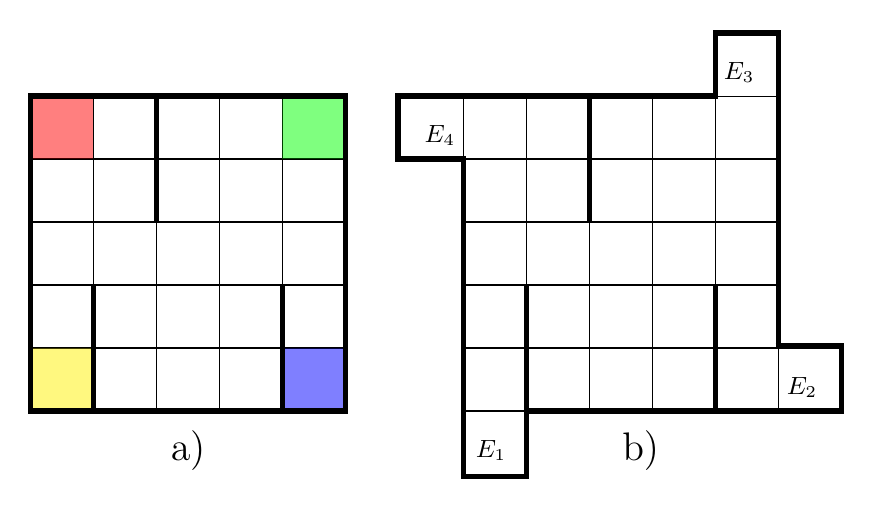
\begin{tikzpicture}
    \newcommand\xoffset{5.5}
    \draw[step=0.8,line width=0.5pt,shift={(0.2,0.2)}] (0.8,0.8) grid (4.8,4.8);

    \draw[line width=0.5pt, fill=yellow, opacity=0.5] (1,1) rectangle (1.8, 1.8);
    \draw[line width=0.5pt, fill=red, opacity=0.5] (1,4.2) rectangle (1.8, 5);
    \draw[line width=0.5pt, fill=blue, opacity=0.5] (4.2,1) rectangle (5, 1.8);
    \draw[line width=0.5pt, fill=green, opacity=0.5] (4.2,4.2) rectangle (5, 5);
    
    \draw[line width=2pt] (1,1) rectangle (5,5);
    \draw[line width=2pt] (1.8,1) -- (1.8,2.6);
    \draw[line width=2pt] (4.2,1) -- (4.2,2.6);
    \draw[line width=2pt] (2.6, 3.4) -- (2.6,5);

    \node at (1.35,1.4) {\LARGE $\text{\person}$};
    \node at (3,2.2) { $\text{\taxi}$};

    \draw[step=0.8,line width=0.5pt,shift={(\xoffset+0.2,0.2)}] (0.8,0.8) grid (4.8,4.8);
    
    %bottom left 
    \draw[line width=2pt, shift={(\xoffset,0)}] (0.965,0.17) -- (1.835,0.17);
    \draw[line width=2pt,shift={(\xoffset,0)}] (1.8,0.17) -- (1.8,2.6); % OK

    % bottom right
    \draw[line width=2pt, shift={(\xoffset,0)}] (5.8,0.965) -- (5.8,1.835);
    \draw[line width=2pt, shift={(\xoffset,0)}] (4.965,1.83) -- (5.835,1.83);

    % top right
    \draw[line width=2pt, shift={(\xoffset,0)}] (5.035,5.8) -- (4.2,5.8);
    \draw[line width=2pt, shift={(\xoffset,0)}] (4.2,5.835) -- (4.2,4.965);

    % top LEFT
    \draw[line width=2pt, shift={(\xoffset,0)}] (0.17,5.035) -- (0.17,4.165);
    \draw[line width=2pt, shift={(\xoffset,0)}] (0.17,4.2) -- (1.035,4.2);

    
    % \draw[line width=2pt, shift={(5.8,0)}] (1.8,1) -- (5.8,1);
    
    
    % \draw[line width=2pt, shift={(\xoffset,0)}] (1,4.2) -- (1,0.17);


    % \draw[line width=2pt,shift={(5.8,0)}] (1,1) rectangle (5,5);
    \draw[line width=2pt, shift={(\xoffset,0)}] (1,4.2) -- (1,0.17); % EAST WALL OK
    \draw[line width=2pt,shift={(\xoffset,0)}] (1.8,1) -- (5.8,1); % SOUTH WALL OK
    \draw[line width=2pt,shift={(\xoffset,0)}] (5,1.8) -- (5,5.8); % WEST WALL OK
    \draw[line width=2pt,shift={(\xoffset,0)}] (4.2,5) -- (0.17,5); % NORTH WALL OK

    % Interior obstacles
    \draw[line width=2pt,shift={(\xoffset,0)}] (4.2,1) -- (4.2,2.6);
    \draw[line width=2pt,shift={(\xoffset,0)}] (2.6, 3.4) -- (2.6,5);
    

    \node[shift={(\xoffset,0)}] at (1.35, 0.5) {\small $E_1$};
    \node[shift={(\xoffset,0)}] at (5.3, 1.3) {\small $E_2$};
    \node[shift={(\xoffset,0)}] at (4.5, 5.3) {\small $E_3$};
    \node[shift={(\xoffset,0)}] at (0.7, 4.5) {\small $E_4$};

    

    
    \node at (3,0.5) {\Large a)};
    \node at (8.75,0.5) {\Large b)};
    \end{tikzpicture}
    \end{adjustbox}
    \end{center}
    \caption{a) }
\label{fig:domain_taxi}
\end{figure}
    

\paragraph{Example 2:} The Taxi domain~\citep{Dietterich2000} is described by three variables: the location of the taxi ($v_1$), and the location and destination of the passenger ($v_2$ and $v_3$). Since the location of the taxi is independent of the other two, it is natural to partition the states according to the location and destination of the passenger. Each partition consists of the possible locations of the taxi, defining a unique equivalent subtask whose terminal states are the locations at which the taxi can pick up or drop off passengers. Since there are 16 valid combinations of passenger location and destination, there are 16 such equivalent subtasks.
\citep{Dietterich2000} calls this condition {\em max node irrelevance}, where ``max node'' refers to a given subtask.

\subsection{Eigenvector Approach}
\label{section:hlmdps_eigenvector_episodic}

If the dynamics $\kernel$ and the state costs $\cR, \cJ$ are known, the power method can be used to solve the original LMDP $\cL$ by composing individual solutions of the subtask LMDPs $\cL_i$.
In this case, the base LMDPs of all equivalence classes are solved by defining Bellman equations in \eqref{eq:eigenvector}.
To compute the values of the original LMDP $\cL$ for the exit states in $\cE$, the compositionality relation in~\eqref{eq:comp3} gives rise to an additional system of linear equations, one for each non-terminal exit state. This additional system of equations can be reformulated in matrix form defined for the exit states ${\bf z}_\cE$:
\begin{equation}\label{eq:exits}
{\bf z}_\cE=G{\bf z}_\cE.
\end{equation}
Here, the matrix $G$ contains the values of the base LMDPs according to~\eqref{eq:comp3}.
The power method can be used on this system of linear equations to obtain the values of all exit states in $\cE$.

\paragraph{Example 1:} In the 4-room example, the row in $G$ corresponding to $\widehat{z}_\cE(2^L)$ contains the element $z^B(2^L)$ in the column for $\widehat{z}_\cE(1^B)$, and the element $z^R(2^L)$ in the column for $\widehat{z}_\cE(1^R)$, while all other elements equal $0$. While the flat approach requires one run of the power method on a large matrix, %of $100\times 100$ states
the hierachical approach needs five runs of the power method on significantly reduced %$(5+4)\times (5+4)$
 matrices (these runs can be parallelized), and one additional run on a $8\times 8$ matrix, corresponding to~\eqref{eq:exits}.\\ %, to obtain the same global optimal solution.

The values of states in $\cS\setminus\cE$ are not explicitly represented since they are given by~\eqref{eq:comp3}.
Since now the value $z(s)$ of each state $s\in\cS$ can be obtained, the optimal policy is directly defined in terms of the values $z$ and~\eqref{eq:lmdp_optimal_policy}. Hence unlike most approaches to hierarchical reinforcement learning, the policy does not select among subtasks, but instead depends directly on the decomposed value estimates.

\subsection{Online and Intra-task Learning}

%Alternatively, in the learning setting where there agent is learning by interacting with the environment, we need to maintain 

In the online learning case, estimates $\widehat{z}_j^1,\ldots,\widehat{z}_j^n$ of the value functions of the base LMDPs associated with each equivalent subtask $\cL_j$ are mantained.These estimates can be updated using the Z-learning rule~\eqref{eqn:zlearning-imp} after each transition.
But to make learning more efficient, a single transition $(s_t,r_t,s_{t+1})$ with $s_t\in\cS_j$ can be used to update the values of {\em all} base LMDPs associated with $\cL_j$ simultaneously. This is known in the literature as intra-task learning~\citep{Kaelbling1993,Jonsson2016}.

%In the case of unknown dynamics, we need to maintain estimates $\widehat{z}_j^1,\ldots,\widehat{z}_j^n$ of the value functions of the base LMDPs associated with each equivalent subtask $\cL_j$. These estimates are updated using the Z-learning rule in~\eqref{eqn:zlearning-imp} after each transition. To make learning more efficient, we can use a single transition $(s_t,r_t,s_{t+1})$ with $s_t\in\cS_j$ to update the values of {\em all} base LMDPs associated with $\cL_j$ simultaneously. This is known in the literature as intra-task learning~\textit{Kaelbling93}.

Given the estimates $\widehat{z}_j^1,\ldots,\widehat{z}_j^n$, then the same system of linear equations in~\eqref{eq:comp3} could be formulated and solved to obtain the value estimates of exit states. However, it is impractical to solve this system of equations every time %the estimates 
$\widehat{z}_j^1,\ldots,\widehat{z}_j^n$ are updated. Instead, estimates $\widehat{z}_\cE$ of the values of exit states in the set $\cE$ are explicitly mantained, and updated incrementally. 
For that,~\eqref{eq:comp3} is turned into an update rule:
\begin{align}\label{eq:comprule}
\widehat{z}_\cE(s) \leftarrow &(1 - \alpha_\ell) \widehat{z}_\cE(s) + \alpha_\ell \sum_{k=1}^n \widehat{z}_j^k(s) \widehat{z}_\cE(\tSi_k).
\end{align}
The question is when to update the value of an exit state. The different alternatives are proposed:
\begin{itemize}
\item[$V_1$:] Update the value of an exit state $s\in\cE_i$ each time the agent takes a transition from $s$.
\item[$V_2$:] When the agent reaches a terminal state of the subtask $\cL_i$, update the values of all exit states in $\cE_i$.
\item[$V_3$:] When the agent reaches a terminal state of the subtask $\cL_i$, update the values of all exit states in $\cE_i$ and all exit states of subtasks in the equivalence class $\cC_j$ of $\cL_i$.
\end{itemize}
Again, the estimated policy $\pi$ is defined directly by the value estimates $\widehat{z}$ and~\eqref{eq:lmdp_optimal_policy}, and thus does not select among subtasks. The pseudo-code of the proposed algorithm is in Algorithm~\ref{alg:online_hlmdps}.

\begin{algorithm}[!htb]
\setstretch{1.2}
% \renewcommand{\thealgorithm}{}
\caption{Online and Intra-Task Learning Algorithm}
\begin{algorithmic}[1]
\State {\bf Input:} An LMDP ${\cL = \langle \cS, \cT, \kernel, \cR, \cJ \rangle}$ and
a partition $\{\cS_i\}_{i=1}^L$ of $\cS$ \newline
A set $\{\cC_1,\ldots,\cC_C\}$ of equivalent subtasks and related base LMDPs $\linebreak\mathcal{L}_j^k = \langle \cS_j, \cT_j, \kernel_j, \cR_j, \cJ_j^k \rangle$

\State {\bf Initialization:} \newline
$\widehat z_\cE(s) := 1 \;\; (\forall s \in \cE)$ \Comment {high-level Z function approximation} \newline
$\widehat z_j^k(s) := 1$ \Comment{base LMDPs $1 \dots |\cT_j|$ for each equivalent subtask $\cL_j$}

\While{$\text{termination condition is not met}$}
%\STATE update all $\alpha_\ell_{\ell}$
\State observe transition $s_t, r_t, s_{t+1} \sim \widehat\pi(\cdot|s_{t})$, where $s_t\in\cS_i$ and $\cL_i\in\cC_j$
%\STATE $\text{update high-level estimation } \widehat z(s_t)$
\State $\text{update lower-level estimations } \widehat z_j^k(s_t)$ \text{using} \eqref{eqn:zlearning-imp}
\If{$s_t$ is an exit or $s_{t+1}$ is terminal for current subtask $\cL_j$}{\;\{$s_t\in\cE$ or $s_{t+1} \in \cT_j$\}}
\State $\text{apply \eqref{eq:comprule} to update $\widehat z_\cE$ using variant } V_1$, $V_2$ or $V_3$
\EndIf
\EndWhile
\State \Return $\widehat z_\cE$ and value functions for the subtasks
\end{algorithmic}
\label{alg:online_hlmdps}
\end{algorithm}
\subsection{Analysis}
Let $\cL=\langle\cS,\cT,\kernel,\cR,\cJ\rangle$ be an LMDP, and let $\cL_i=\langle\cS_i,\cT_i,\kernel_i,\cR_i,\cJ_i\rangle$ be a subtask associated with the partition $\cS_i\subseteq\cS$. Let $z$ denote the optimal value of $\cL$, and let $z_i$ denote the optimal value of $\cL_i$.

\begin{lemma}\label{lemma:same}
If the reward of each terminal state $\tSi\in\cT_i$ equals its optimal value in $\cL$, i.e.~$z_i(\tSi)=z(\tSi)$, the optimal value of each non-terminal state $s\in\cS_i$ equals its optimal value in $\cL$, i.e.~$z_i(s)=z(s)$.
\end{lemma}

\begin{proof}
Since $\kernel_i$ and $\cR_i$ are the restriction of $\kernel$ and $\cR$ onto $\cS_i$, then for each $s\in\cS_i$ 
\begin{align*}
    z_i(s) &= e^{\cR_i(s)/\lambda} \sum_{s'}\kernel_i(s'|s)z_i(s') \\
    &= e^{\cR(s)/\lambda} \sum_{s'}\kernel(s'|s)z_i(s'),
\end{align*}
which is %exactly
 the same Bellman equation as for $z(s)$.
Since $z_i(\tSi)=z(\tSi)$ for each terminal state $\tSi\in\cT_i$, $z_i(s)=z(s)$ is immediately obtained for each non-terminal state $s\in\cS_i$.
\end{proof}
As a consequence of Lemma~\ref{lemma:same}, assigning the optimal value $z(\tSi)$ to each exit state $\tSi\in\cE$ yields a solution to~\eqref{eq:exits}, which is thus guaranteed to have a solution with eigenvalue~$1$. Lemma~\ref{lemma:same} also guarantees that \eqref{eq:comp3} can be used to compute the optimal value of any arbitrary state given optimal values of the base LMDPs and the exit states. The only necessary conditions needed for convergence to the optimal value function is that $(i)$ $\{\cS_i\}_{i=1}^L$ is a proper partition of the state space; and $(ii)$ the set of terminal states $\cT_i$ of each subtask $\cL_i$ includes all states reachable in one step from $\cS_i$.

%\setcounter{lemma}{0}

%\setcounter{\xlemma}{0}
\begin{lemma}
The solution to \eqref{eq:exits} is unique.
\end{lemma}

\begin{proof}
By contradiction. Assume that there exists a solution ${\bf z}_\cE'$ which is different from the optimal values ${\bf z}_\cE$. Then ${\bf z}$ and ${\bf z}'$ can be extended to all states in $\cS$ by applying \eqref{eq:comp3}. Due to the same argument as in the proof of Lemma~\ref{lemma:same}, the solution ${\bf z}'$ satisfies the Bellman optimality equation of all states in $\cS$. Hence ${\bf z}'$ is an optimal value function for the original LMDP $\cL$, which contradicts that ${\bf z}'$ is different from ${\bf z}$ since the Bellman optimality equations have a unique solution.
\end{proof}

\begin{lemma}
For each subtask $\cL_i$ and state $s\in\cS_i^+$, it holds that $z_i^1(s)+\cdots+z_i^n(s)\leq 1$.
\end{lemma}

\begin{proof}
By induction. The base case is given by terminal states $t_\ell\in\cT_i$, in which case $z_i^1(t_\ell)+\cdots+z_i^n(t_\ell) = z_i^\ell(t_\ell) = 1$. For $s\in\cS_i$, the Bellman equation for each base LMDP yields
\begin{align*}
    \sum_{k=1}^n z_i^k(s)=e^{\cR_i(s)/\lambda}\sum_{s'}\kernel(s'|s)\sum_{k=1}^n z_i^k(s').
\end{align*}


Since $\cR_i(s)=\cR(s)<0$ holds by assumption, and since $z_i^1(s')+\cdots+z_i^n(s')\leq 1$ holds for each $s'$ by hypothesis of induction, it follows that $z_i^1(s)+\cdots+z_i^n(s)\leq 1$.
\end{proof}
As a consequence, just like the matrix $RP$ in \eqref{eq:eigen_lmdp}, the matrix $G$ in \eqref{eq:exits} has spectral radius at most $1$, and hence the power method is guaranteed to converge to the unique solution with largest eigenvalue $1$, corresponding to the optimal values of the exit states.

The convergence rate of the power method is exponential in $\gamma<1$, the eigenvalue of $RP$ or $G$ with second largest value and independent of the state space.
The average running time scales linearly with the number of non-zero elements in $RP$ or $G$~\citep{Todorov2006}, which is drastically reduced compared to the non-hierarchical approach. 
%Assuming a similar convergence rate, the time complexity of the power method depends on the matrix multiplication.
More precisely, given an upper bound $B$ on the support of $\kernel$ and a sparse representation, the matrix multiplication in~\eqref{eq:eigen_lmdp} has complexity $\mathcal{O}(BS)$. In comparison, the matrix multiplication of the $\mathcal{O}(CN)$ base LMDPs has complexity $\mathcal{O}(BK)$, while the matrix multiplication in \eqref{eq:exits} has complexity $\mathcal{O}(NE)$. Hence the hierarchical approach is competitive whenever $\mathcal{O}(CNBK+NE)$ is smaller than $\mathcal{O}(BS)$. In a $10\times 10$-room example, $CNBK+NE=500+1{,}805=2{,}305$, while $BS=10{,}000$.

%The convergence rate of the power iteration method is $\lambda<1$, where $\lambda$ is the eigenvalue of $RP$ or $G$ with second largest value, i.e.~less than $1$. Assuming a similar convergence rate, the time complexity of the power iteration method depends on the matrix multiplication. Given an upper bound $B$ on the support of $P$ and a sparse representation, the matrix multiplication in~\eqref{eq:matrixz} has complexity $O(BS)$. In comparison, the matrix multiplication of the $O(CN)$ base LMDPs has complexity $O(BK)$, while the matrix multiplication in \eqref{eq:exits} has complexity $O(NE)$. Hence the hierarchical approach is competitive whenever $O(CNBK+NE)$ is smaller than $O(BS)$. In the $10\times 10$ room example, $CNBK+NE=500+1{,}805=2{,}305$, while $BS=10{,}000$.

\section{Experiments}
\label{section:hlmdps_experiments}
This section contains the evaluation of the learning algorithm in the two classic control problems introduced.\footnote{Code available at https://github.com/guillermoim/HRL\_LMDP}
% Vicenc:
% \footnote{texttt{https://github.com/guillermoim/HRL\_LMDP}}
%, the Rooms domain and the Taxi domain.
The objective of this evaluation is to analyze empirically the different update alternatives ($V_1$, $V_2$, and $V_3$), and
to compare against a flat approach which exploits the benefits of LMDPs without the hierarchy (Z-IS), and the hierarchical approach based on options ($Q_o$)~\citep{Sutton1999} that was introduced in section~\ref{section:options}. The main goal is to empirically demonstrate that the approach here presented is more sample efficient than the other algorithms. Each algorithm is run with four different random seeds to analyze the (normalized) average MAE (mean absolute error) against the optimal value function (computed separately) and its standard deviation over the number of samples. Since the value functions are different for Q-learning and LMDP methods, the self-normalized MAE (Figures \ref{fig:hlmdps_errors_nrooms} and \ref{fig:hlmdps_errors_taxi}) for different configurations and domains is reported instead. Further, for a fair comparison between approaches, only the exit set is used for calculating the MAE.

%In this section, we empirically test the model-free algorithm in several experiments. In the first set of experiments, we extend the example from Figure~\ref{fig:ex} to $X\times Y$ rooms. In the second set of experiments, we use the Taxi domain~\textit{dietterich2000hierarchical}.

In all experiments, the learning rates for each abstraction level is $\alpha_\ell(t) = c_\ell / (c_\ell + n)$ where $n$ represents the episode each sample $t$ belongs to. The constant $c_\ell$ is empirically optimized for each domain. For LMDPs, a temperature $\eta=1$ is used, which provides good results. $Q_o$ solves an equivalent MDP with {\em deterministic} actions, which should actually give it an advantage. For fairness, $Q_o$ obtains the same per-step negative reward, exploits the same equivalence classes, learns the same subtasks (i.e.~reach a terminal state), and has knowledge of which options are available in each state.

In addition, the MAE for the subtasks learning is also reported. The intention for this is two-fold: first, to show that the value functions for the subtasks also converge to their optimal value, and second, that the faster learning of the subtasks boost the speed of the learning at the higher level.

\subsection{N-room domain.}
Here performance for different room sizes and number of rooms (Figure \ref{fig:hlmdps_errors_nrooms}) is presented. In all configurations the proposed hierarchical approach outperfoms Z-IS and $Q_o$. Concretely, $Q_o$ suffers from non-stationarity: initial option executions will incur more negative reward than later executions, which causes high-level Q-learning updates to be {\em incorrect}, and it takes the learner significant time to recover from this.

\begin{figure}[!htb]
\centering
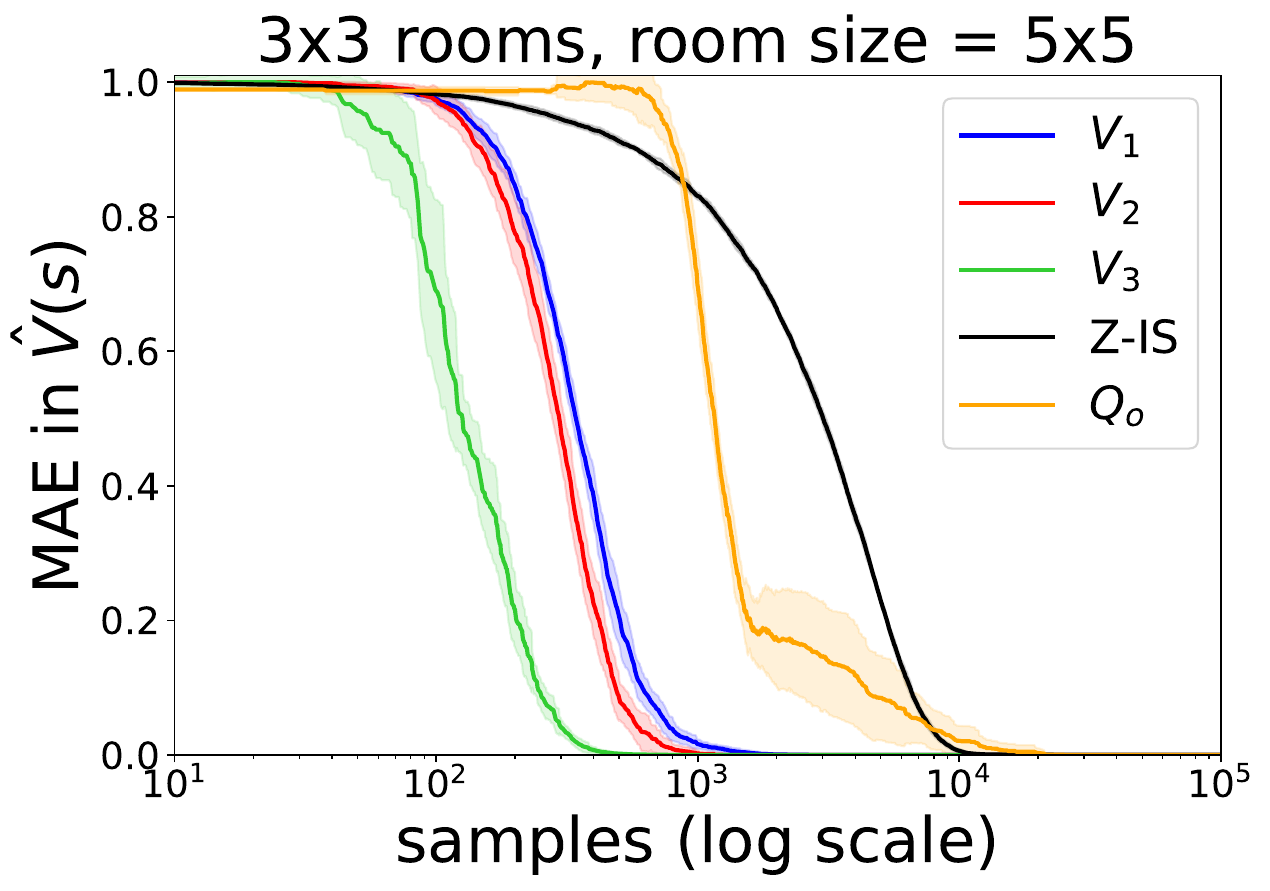
\includegraphics[width=0.32\textwidth]{figures/chapter1/learning/nrooms_3_3.pdf}
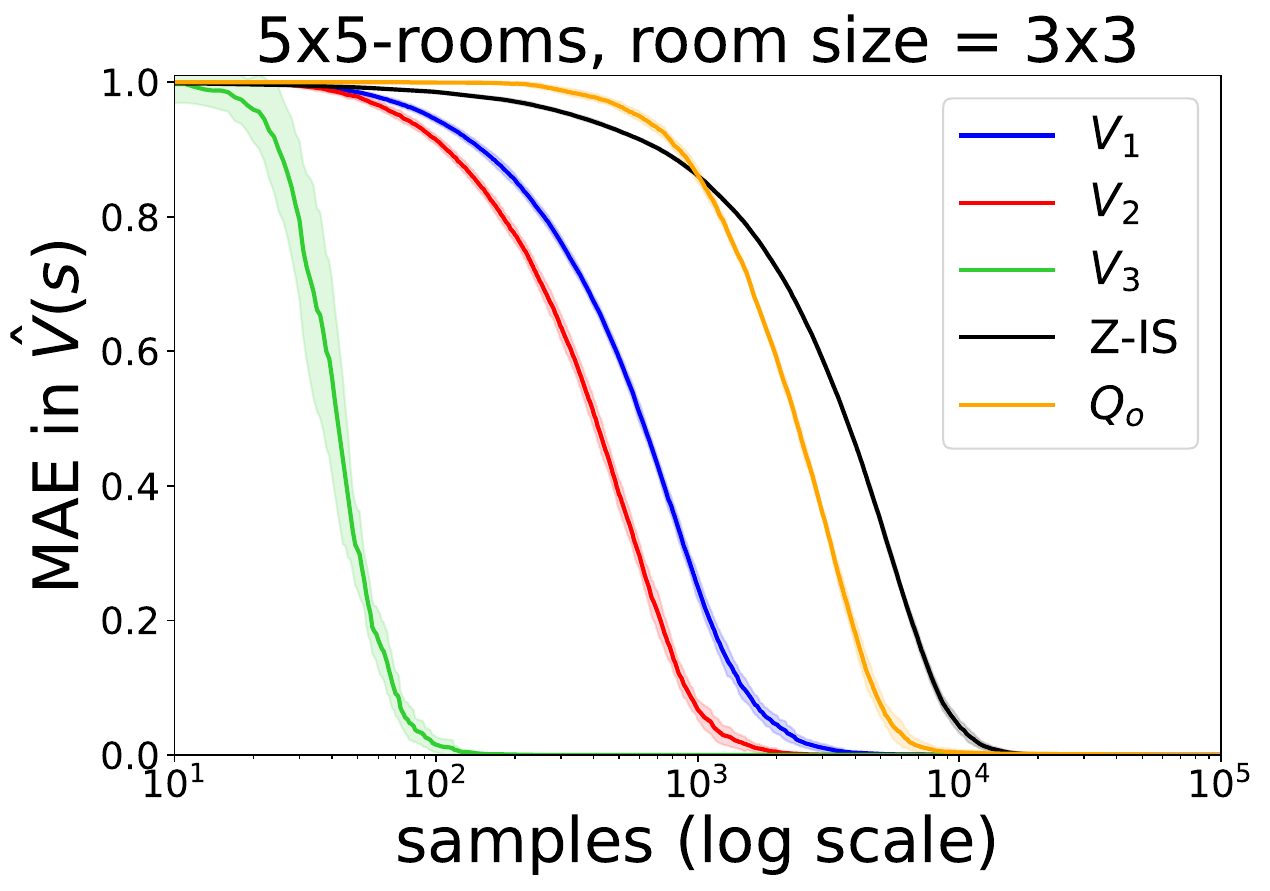
\includegraphics[width=0.32\textwidth]{figures/chapter1/learning/nrooms_5_5.pdf}
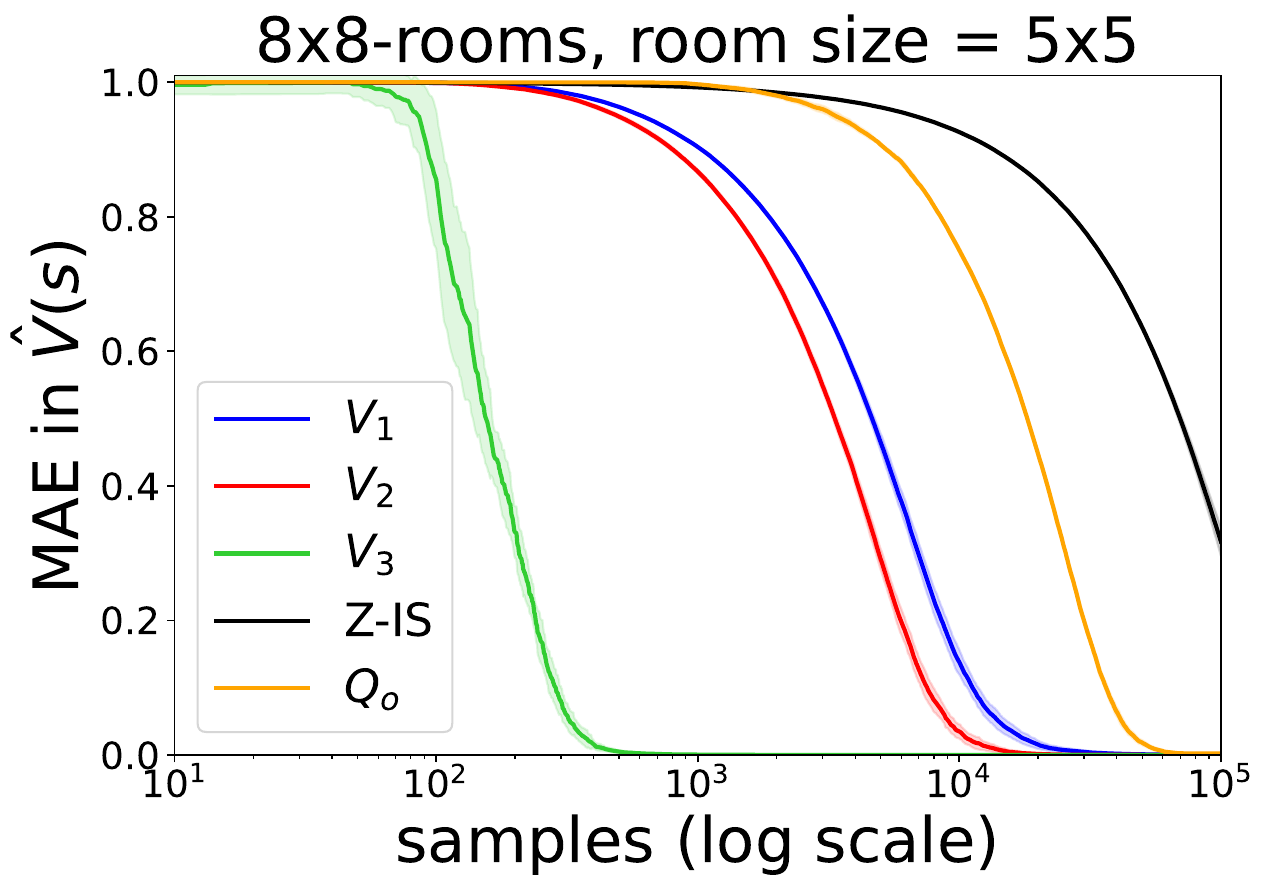
\includegraphics[width=0.32\textwidth]{figures/chapter1/learning/nrooms_8_8.pdf}
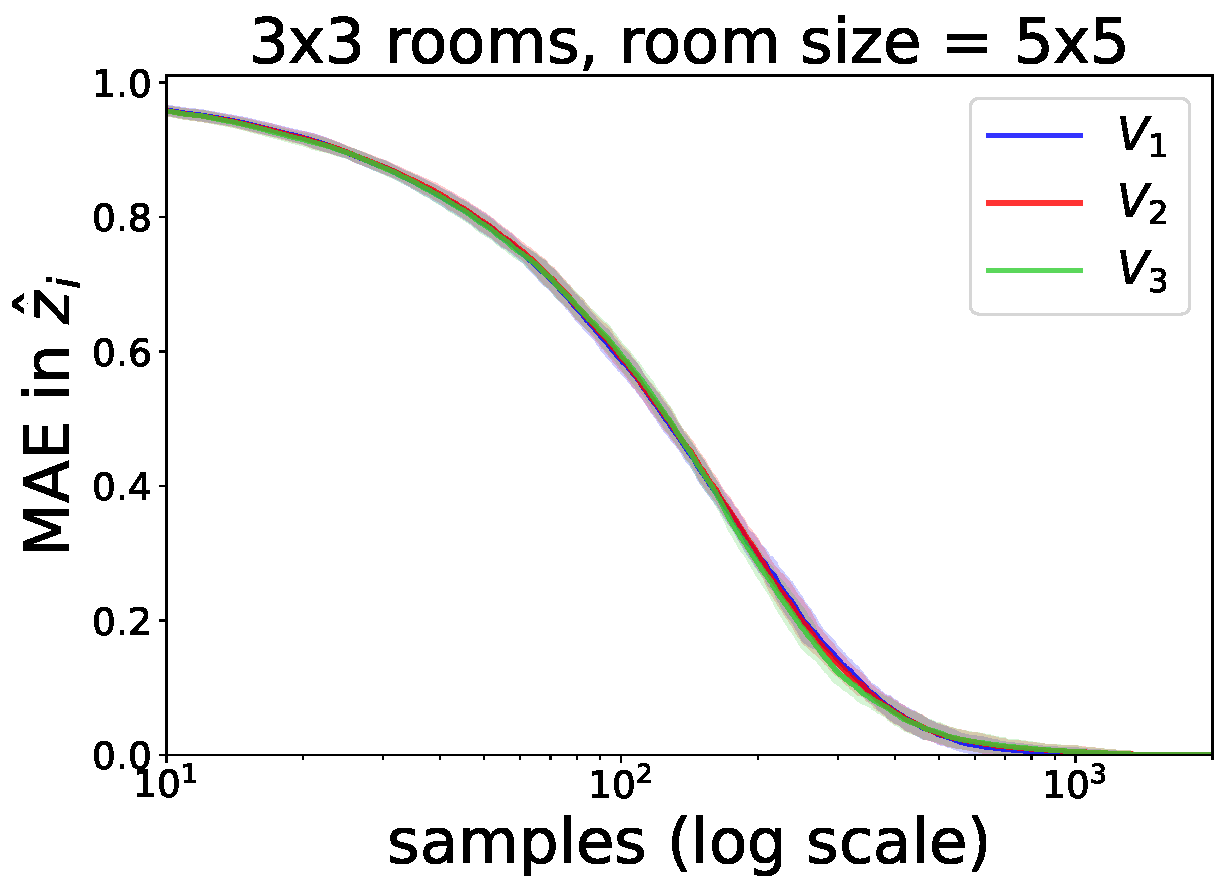
\includegraphics[width=0.32\textwidth]{figures/chapter1/subtasks/nrooms_3_3_subtasks.pdf}
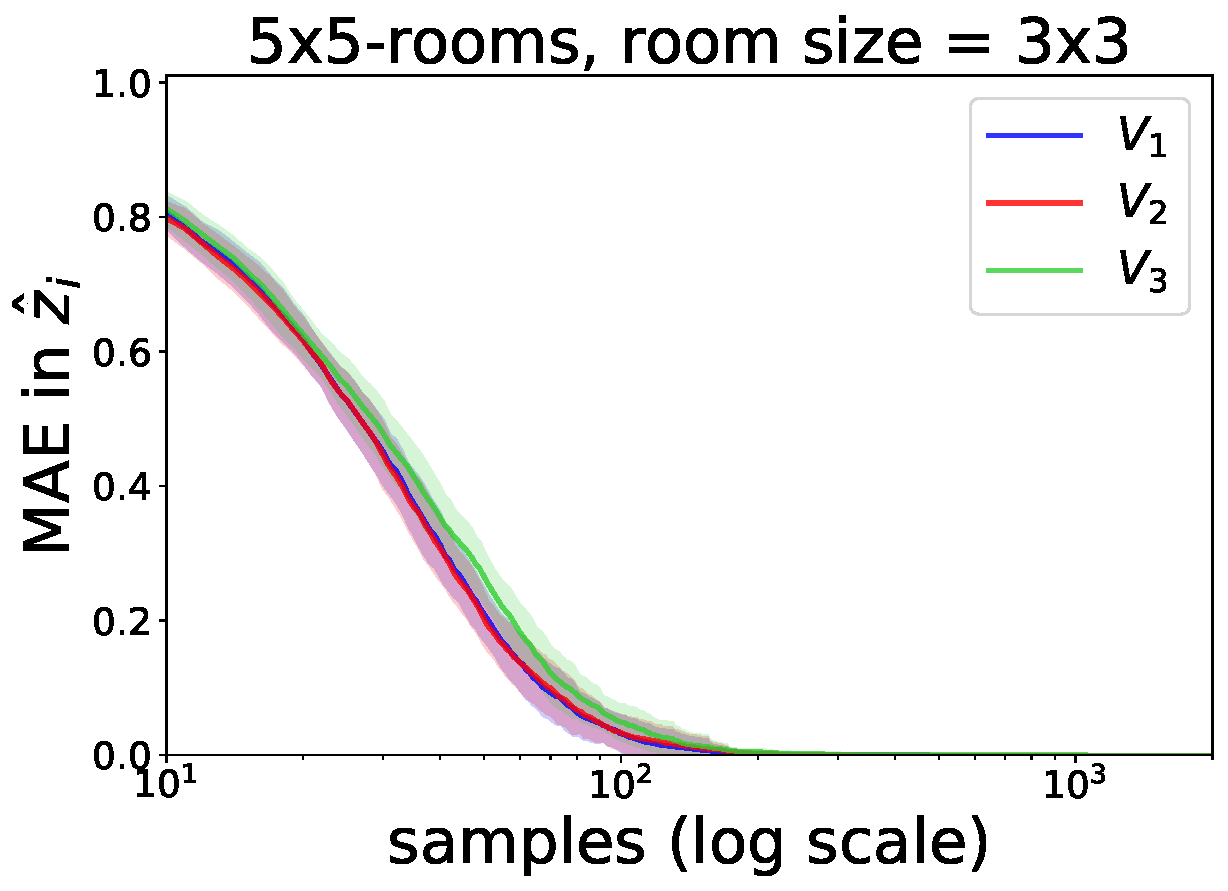
\includegraphics[width=0.32\textwidth]{figures/chapter1/subtasks/nrooms_5_5_subtasks.pdf}
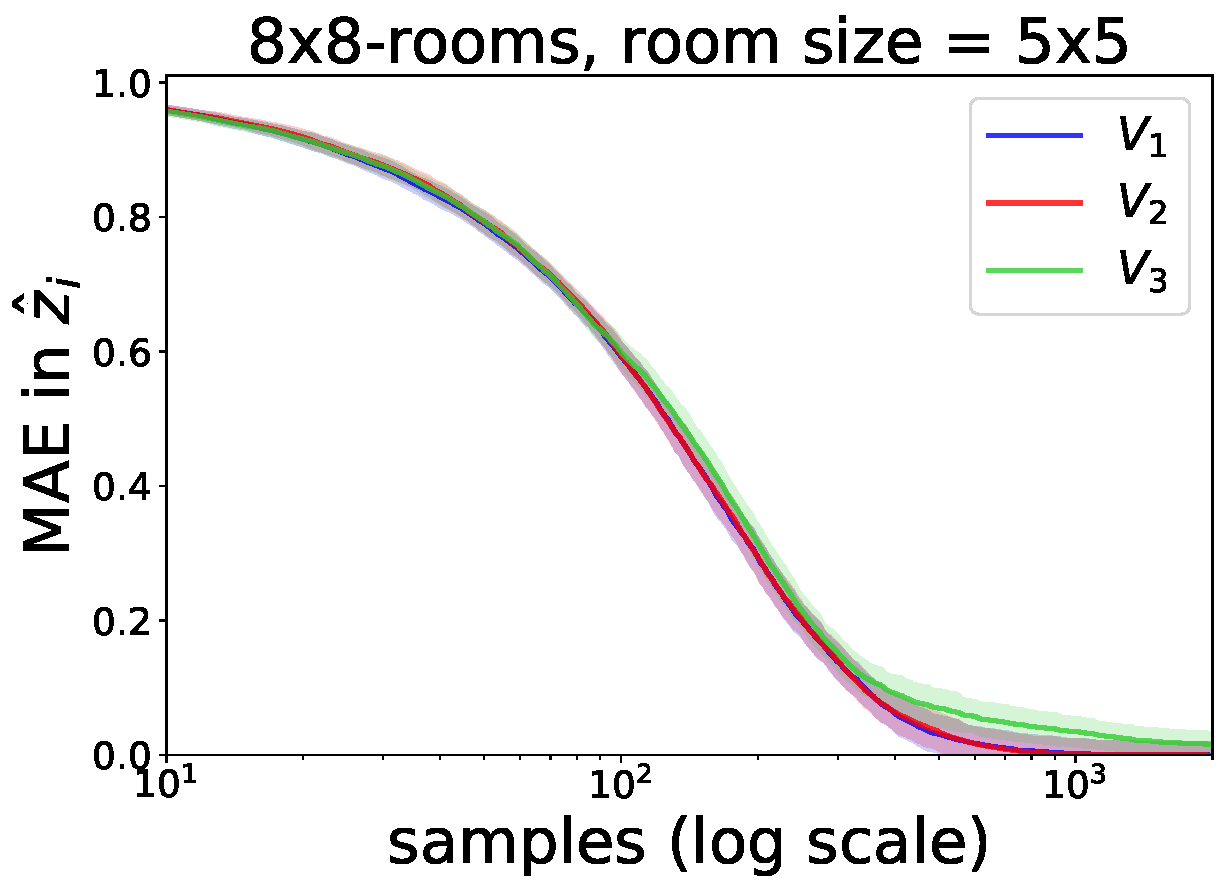
\includegraphics[width=0.32\textwidth]{figures/chapter1/subtasks/nrooms_8_8_subtasks.pdf}
\caption{ Results for $3\times 3$ rooms of size $5 \times 5$ (left);
$5\times 5$ rooms of size $3 \times 3$ (center); $8 \times 8$ rooms of size $5\times 5$ (right).}
%; and d) $5 \times 5$ with Q-learning ($Q_o$).}
\label{fig:hlmdps_errors_nrooms}
\end{figure}

Figure~\ref{fig:hlmdps_errors_nrooms} (left) shows results for $3\times 3$ rooms of size $5\times 5$ and Figure~\ref{fig:hlmdps_errors_nrooms} (center) shows results for $5\times 5$ rooms of size $3\times 3$. Both scenarios have $225$ interior states.
The difference between variants $V_1$, $V_2$ and $V_3$ is more pronounced in the second case, when the number of subtasks increases (more rooms) and the partition for each subtask is smaller (smaller rooms). Figure~\ref{fig:hlmdps_errors_nrooms} (right) shows how the method scales with the number of rooms of size $5\times 5$.
Again, variant $V_3$ has the best performance, in this case by a larger 
margin than before.

% Vicenc:
%Figure~\ref{fig:hlmdps_errors_nrooms} (left) shows results for $3\times 3$ rooms of size $5\times 5$ and Figure~\ref{fig:hlmdps_errors_nrooms} (center) shows results for $5\times 5$ rooms of size $3\times 3$. Both scenarios have $225$ interior states.
%The difference between variants $V_1$, $V_2$ and $V_3$ is more pronounced in the second case, when the number of subtasks increases (more rooms) and the partition for each subtask is smaller (smaller rooms). Figure~\ref{fig:hlmdps_errors_nrooms} (right) shows results for a larger number of rooms of size $5\times 5$. The variant $V_3$ has the best performance, in this case by a larger margin than before.



% Variant $V_3$, updating the exits of all equivalent rooms, converges the fastest, and the difference increases as a function of the number of rooms.

%We run several experiments with different grid sizes. One one side, we kept the room dimensions fixed to $5 \times 5$ to analyze the impact of the number of rooms in two grids of $3 \times 3$ ($246$ states) and $8 \times 8$ ($1696$ states). Alternatively, we reduced the size of individual rooms to $3\times3$ and increased the number of rooms to $5 \times 5$ ($270$ states). The first and the last instances have the same number ($225$) of interior states. This allows us to have a better understanding of different  hierarchical structures.

%In each problem, we run the three variants of the model-free algorithm ($V_1$, $V_2$, $V_3$) and Z-learning without hierarchical decomposition (Z-IS). 


\subsection{Taxi Domain.}
%Since LMDPs have no explicit actions, we adapted the Taxi domain as follows.
To allow comparison between all the methods, we adapted the Taxi domain as follows: when the taxi is at the correct pickup location, it can transition to a state with the passenger in the taxi.
In a wrong pickup location, it can instead transition to a terminal state with large negative reward (simulating an unsuccessful pick-up).
When the passenger is in the taxi, it can be dropped off at any pickup location, successfully completing the task whenever dropped at the correct destination.

\begin{figure}[!h]
\centering
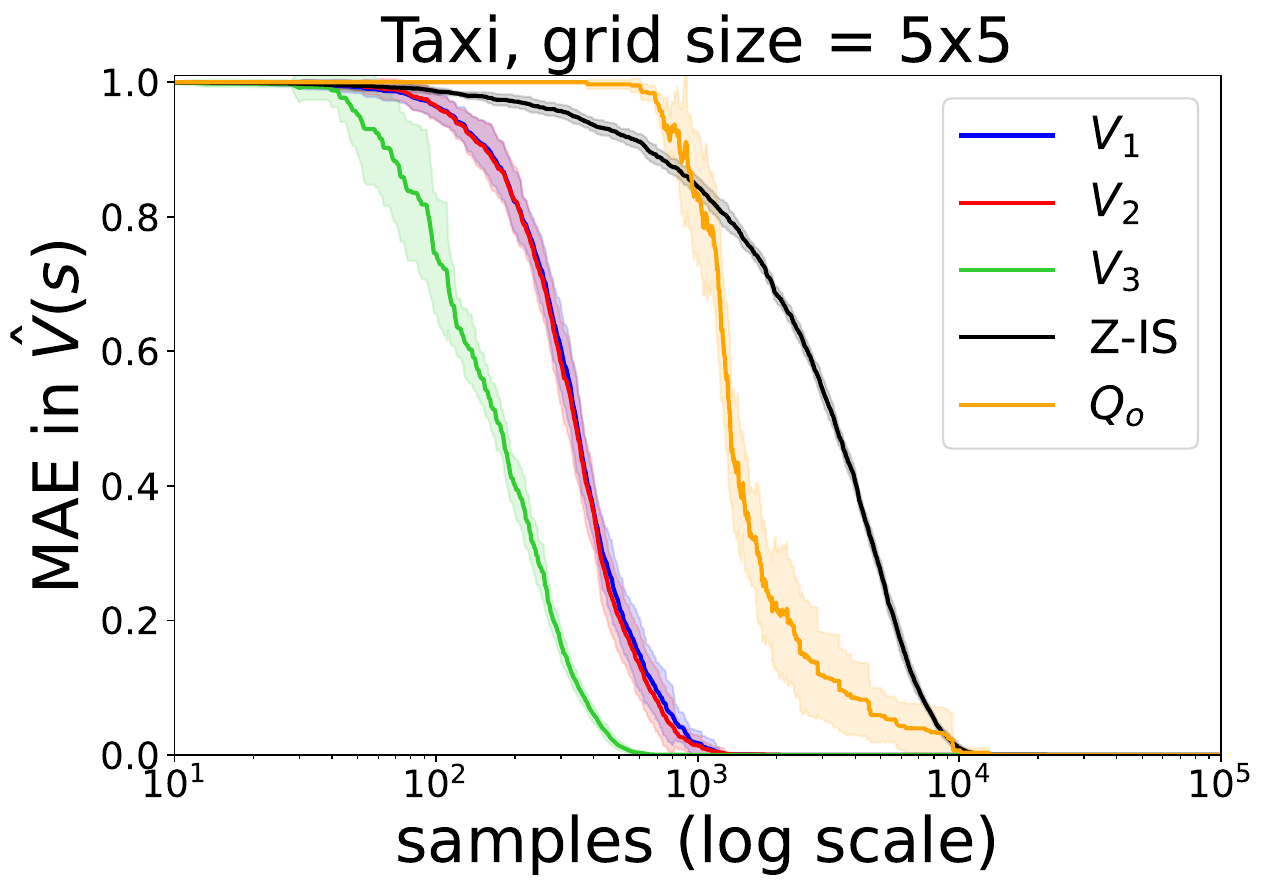
\includegraphics[width=0.49\textwidth]{figures/chapter1/learning/taxi_5.pdf}
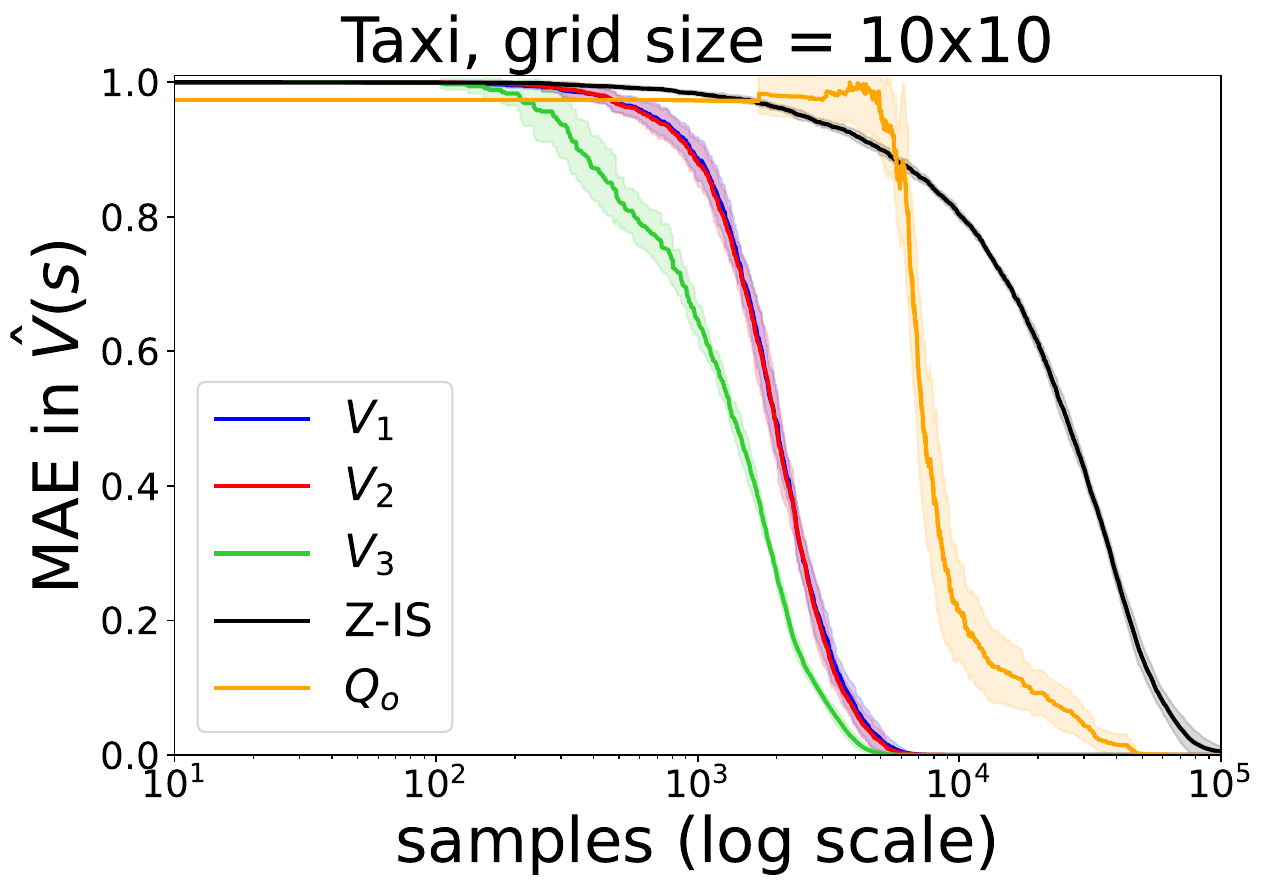
\includegraphics[width=0.49\textwidth]{figures/chapter1/learning/taxi_10.pdf}
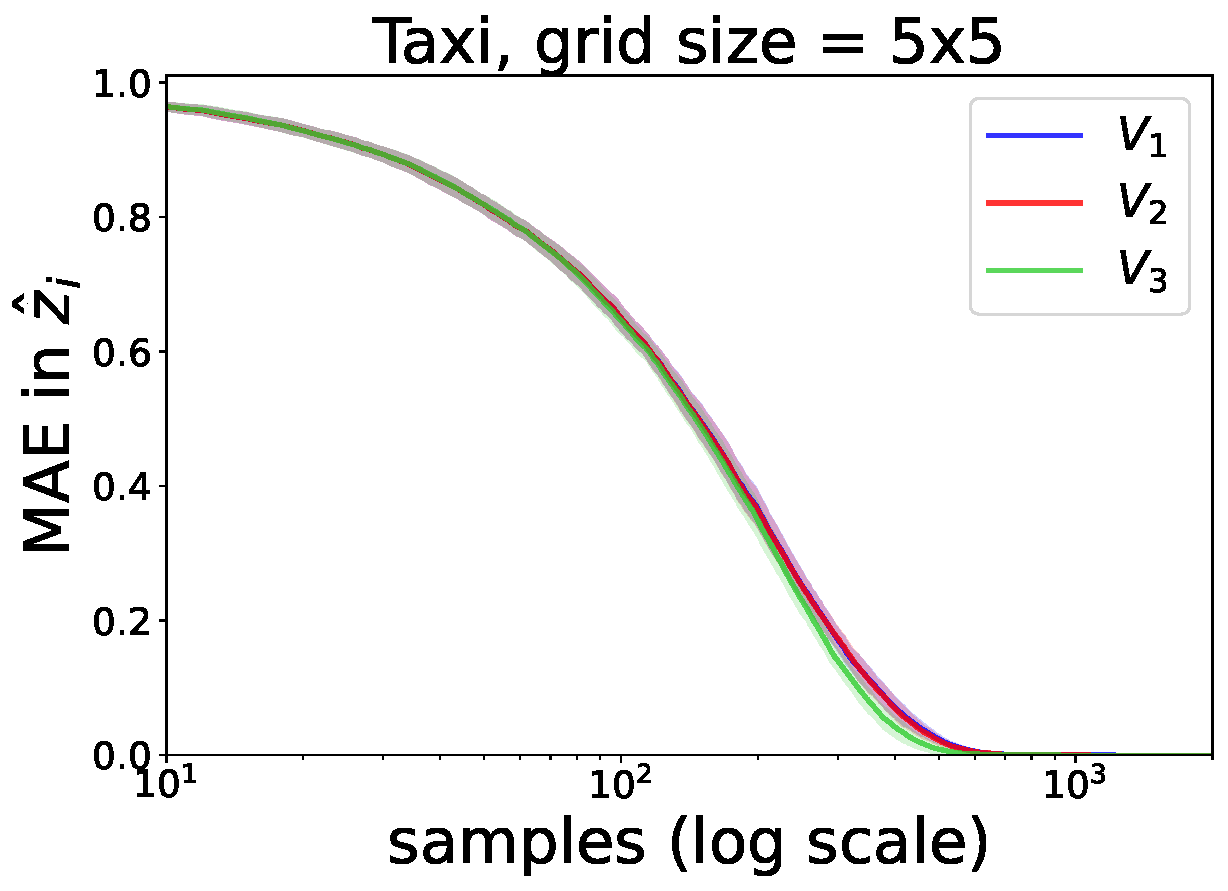
\includegraphics[width=0.49\textwidth]{figures/chapter1/subtasks/taxi_5_subtasks.pdf}
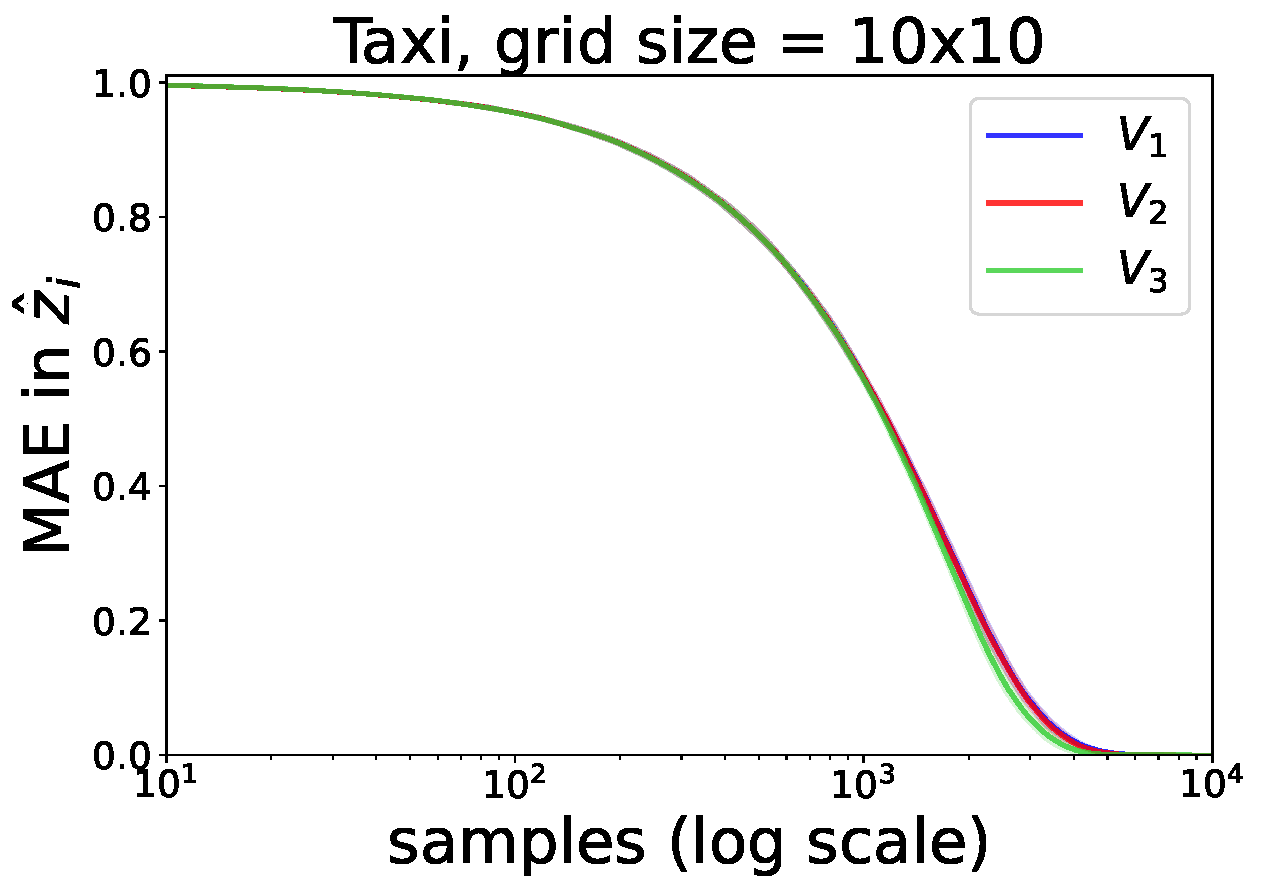
\includegraphics[width=0.49\textwidth]{figures/chapter1/subtasks/taxi_10_subtasks.pdf}
\caption{Results for $5 \times 5$ (left) and $10 \times 10$ (right) grids of Taxi domain.}
\label{fig:hlmdps_errors_taxi}
\end{figure}

%\begin{figure}[H]
%\centering
%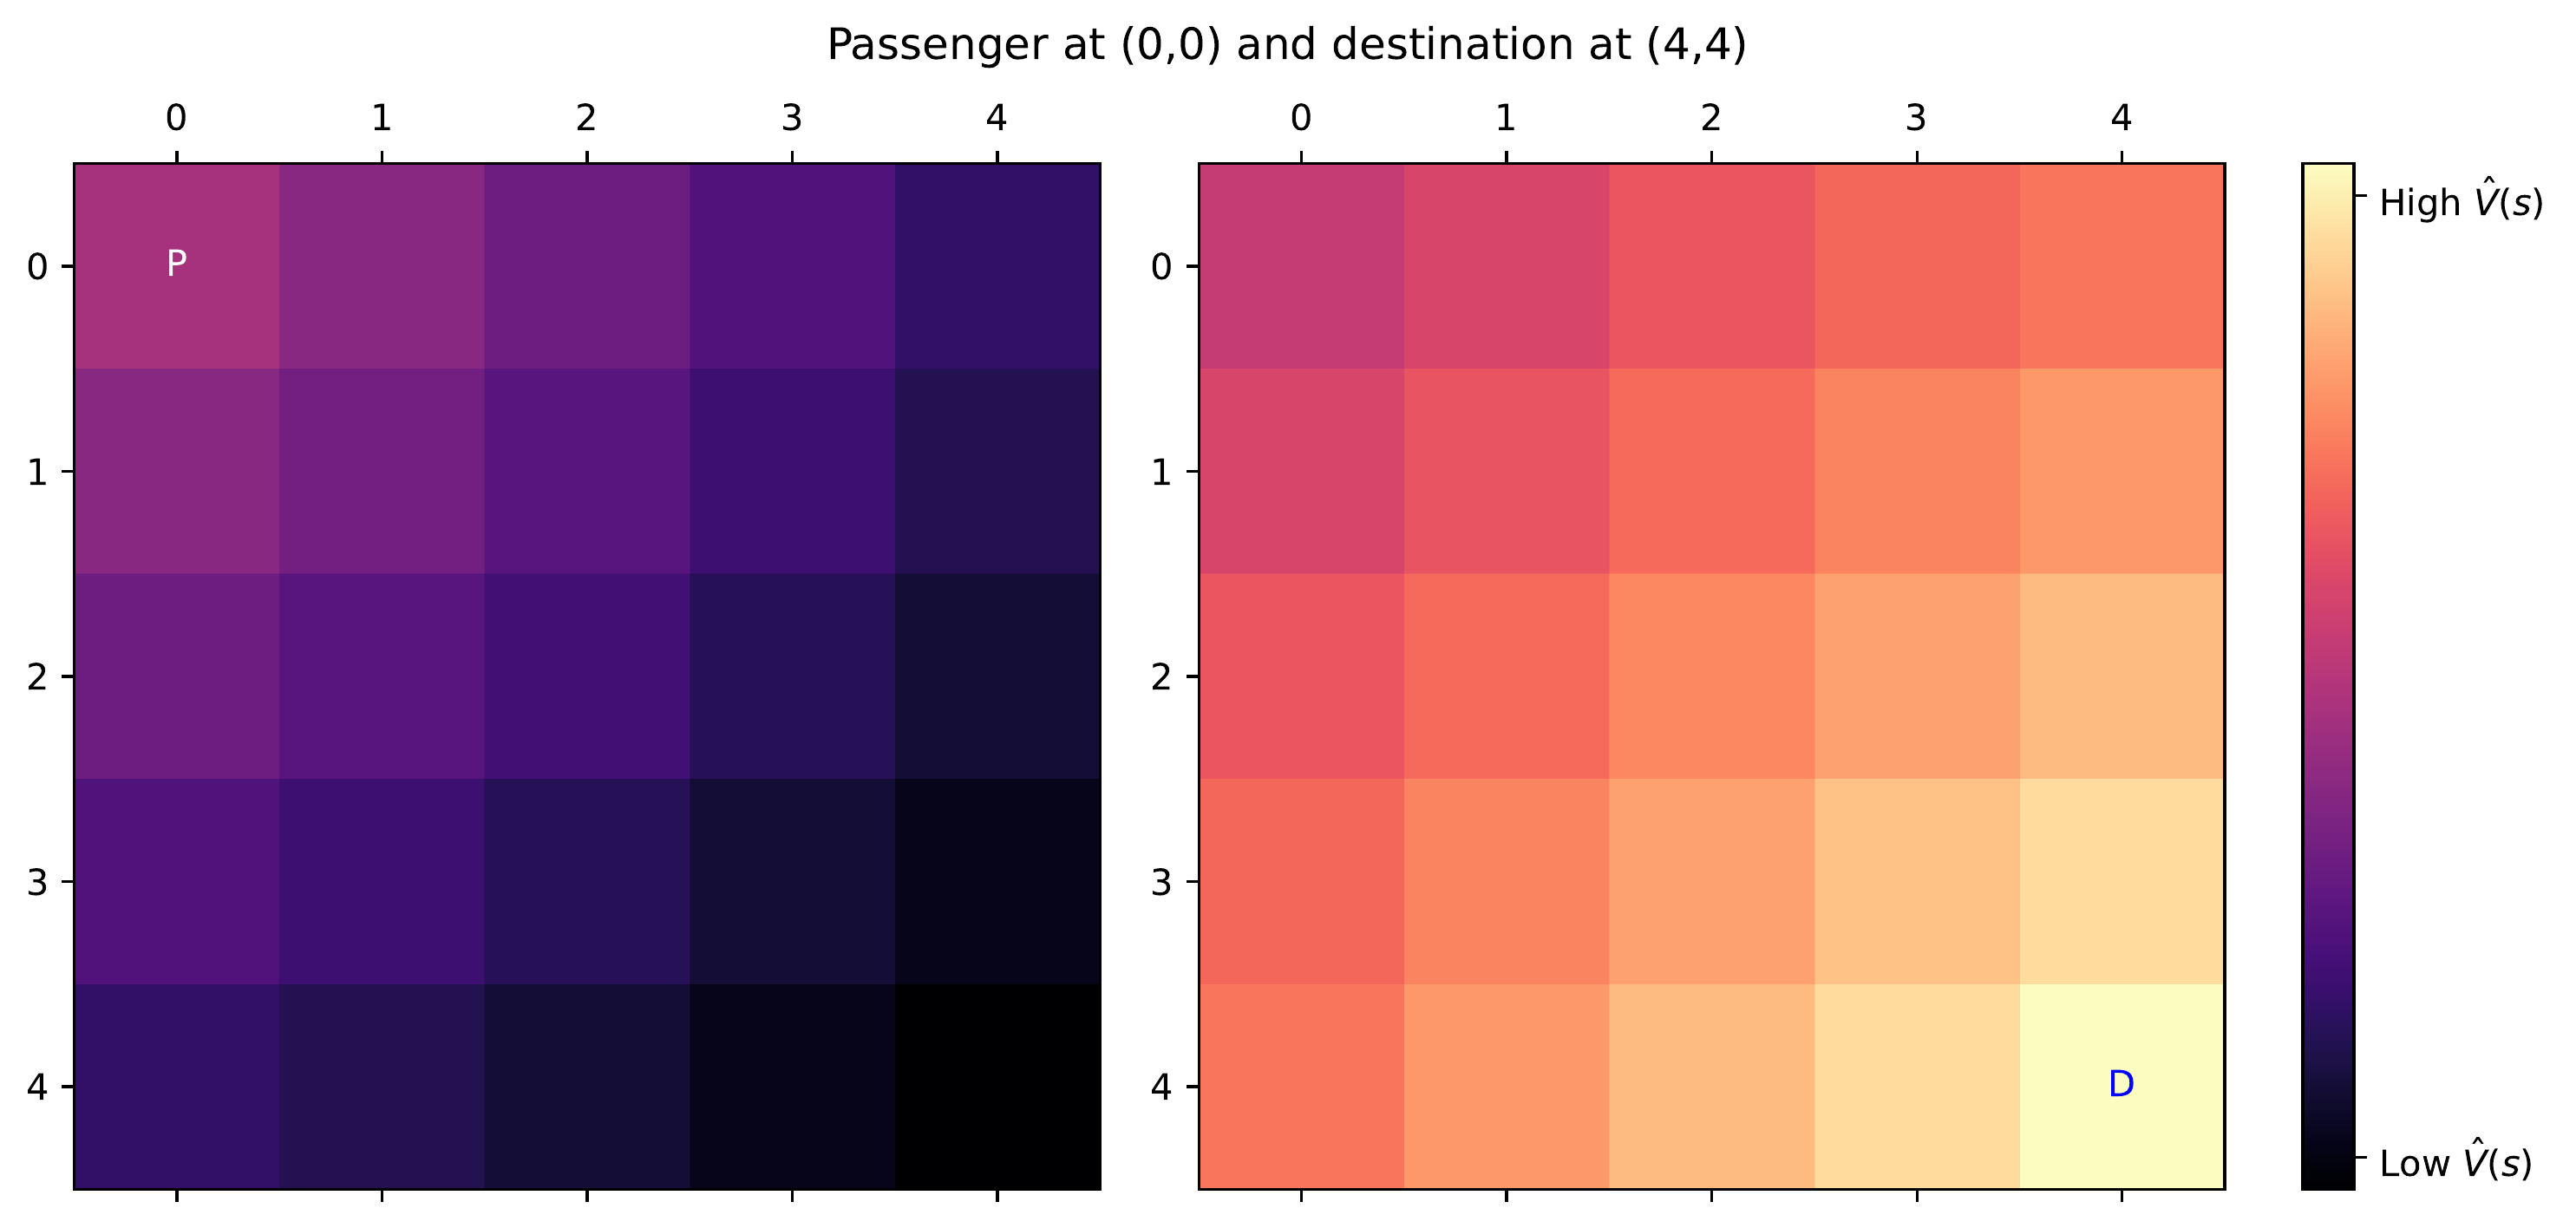
\includegraphics[scale=0.3]{Figures/taxi_dom_VF.png}
%\caption{$\widehat v(s)$ in a $5 \times 5$ Taxi, passenger (\textit{P}) and destination (\textit{D}).}
%\label{fig:taxi_VF}
%\end{figure}

%the pickup corner is an exit state connected to the partition in which the passenger is on the taxi (and, thus, can be moved to the destination) while the other corners are non-goal terminal states. This way, the agent can drop the passenger at any corners, but it will only successfully terminate the episode in the specified destination. If we disentangle the state space we can represent the value function graphically as in figure \ref{fig:taxi_VF}. In this domain, subtasks are to optimally go to the corners.
%\vspace{-0.1em}
Figure~\ref{fig:hlmdps_errors_taxi} shows results in two instances of size $5 \times 5$ ($408$ states) and $10 \times 10$ ($1608$ states). %, respectively.
Again, the proposed hierarchical approach outperforms Z-IS and $Q_o$.
In this case, the difference between $V_1$, $V_2$ and $V_3$ is less pronounced, even when the grid size increases. One possible explanation is the small number of exit states in this problem.

%Figures \ref{fig:hlmdps_errors_nrooms} and \ref{fig:hlmdps_errors_taxi} show the Mean Absolute Error (MAE) measured on $\widehat v(s)$ against the optimal value function $v^*(s)$ previously computed using the power iteration method. Clearly, our approach outperforms the flat version of Z-learning. Regarding the gridworld domain (figure \ref{fig:hlmdps_errors_nrooms}) it is observed that the three variants of our algorithm perform similarly for the case of the $3\times3$ grid. However, when the number of rooms is increased ($5\times5$ and $8\times8$ ) and thus, the hierarchical structure can be better exploited, each of the more sophisticated approaches improves the previous one. As for the Taxi domain (figure \ref{fig:hlmdps_errors_taxi}) the three versions converge much faster than flat learning, but yield similar results. In this case, the structure of the partitions (most of them have a single exit state) is the reason that further assumptions do not necessarily improve the performance as the three variants comprise the same effects.

\section{Discussion and Conclusion}

In this paper we have introduced a novel approach to hierarchical reinforcement learning that focuses on the class of linearly-solvable Markov decision processes.
Using subtask compositionality, we can decompose the value function and derive algorithms that converge to the optimal value function.
To the best of our knowledge, our approach is the first to exploit both the concurrent compositionality enabled by LMDPs together with hierarchies and intra-task learning to obtain globally optimal policies efficiently.

The proposed hierarchical decomposition leads to a new form of zero-shot learning that allows to incorporate subtasks that belong to an existing equivalent class without additional learning effort.
For example, adding new rooms in our example.
This is in contrast with existing methods that only exploit linear compositionality of tasks.

Our approach is limited to OR compositionality of subtasks, but there is no fundamental limitation that prevents arbitrary compositions.
The benefits of hierarchies can be combined for example, with the extended value functions proposed in~\citep{NangueTasse2020}.